\section{Kit de Clasificación Completo}

La integración de todos los subsistemas diseñados (mecánico, neumático, de control, de visión y eléctrico) resulta en un kit educativo compacto y funcional para enseñanza de robótica, visión por computador y ROS2. La Figura \ref{fig:kitCompleto} presenta el ensamblaje completo del kit con todos sus componentes principales.

\begin{figure}[H]
    \centering
    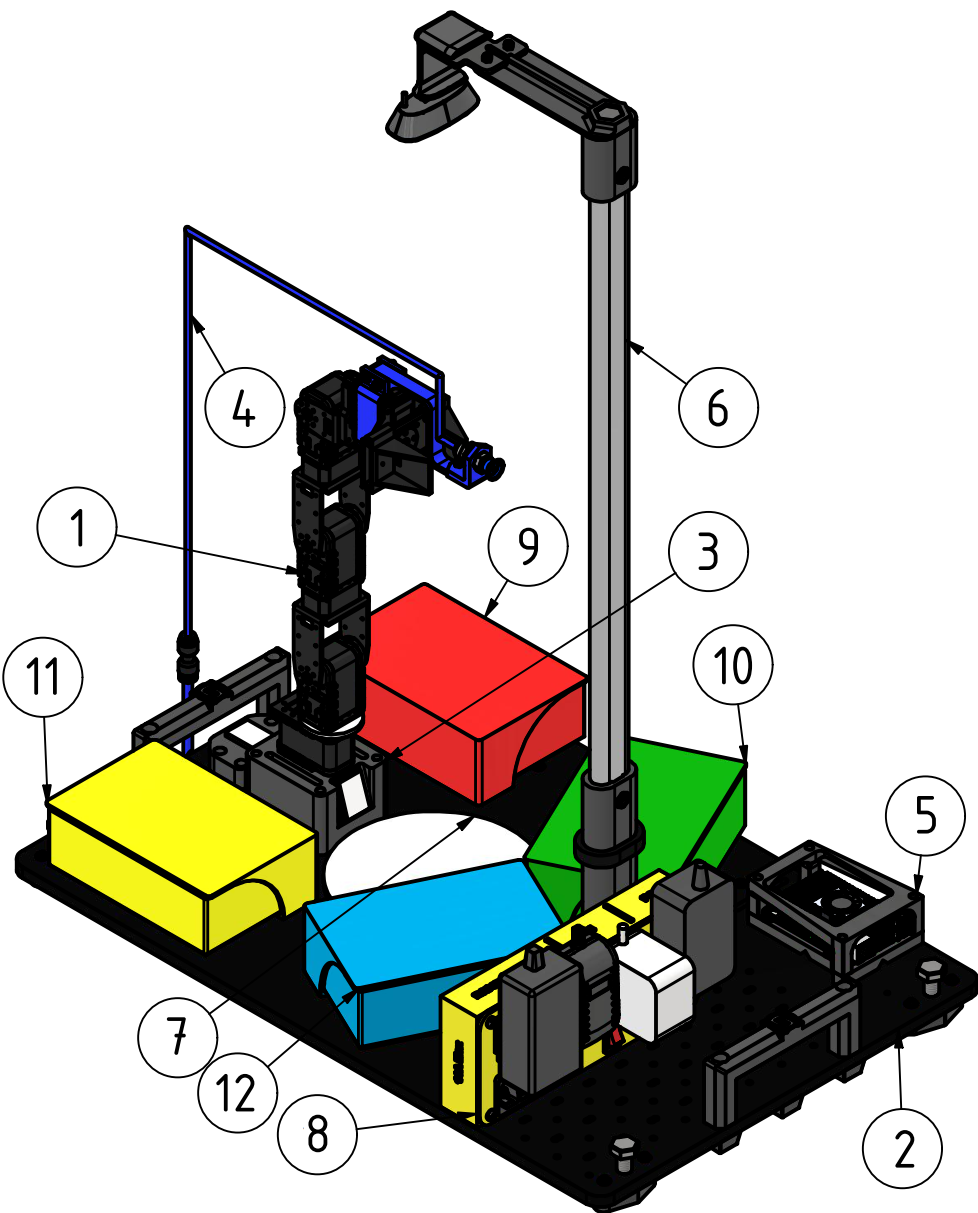
\includegraphics[width=0.9\textwidth]{06disenoConceptual/img/kit.png}
    \caption{Kit de clasificación completo ensamblado. (1) Manipulador robótico PhantomX Pincher AX-12 con 4 grados de libertad, (2) Plataforma base de MDF (554 mm × 360 mm × 9 mm) con acabado negro mate, (3) Base del manipulador con sistema de identificación numérica, (4) Sistema de succión por vacío con gripper intercambiable, (5) Controlador Raspberry Pi 5 en carcasa protectora, (6) Soporte de cámara con mástil vertical y brazo en voladizo, (7) Zona de recolección circular blanca (Ø146 mm), (8) Multitoma personalizada con control individual de subsistemas, (9) Caneca de depósito roja, (10) Caneca de depósito verde, (11) Caneca de depósito azul, (12) Caneca de depósito amarilla. Todos los componentes se integran en contenedor plástico de 600 mm × 400 mm para almacenamiento y transporte.}
    \label{fig:kitCompleto}
\end{figure}

\subsection{Componentes Principales del Kit}

El kit integrado está compuesto por los siguientes subsistemas y componentes principales:

\begin{table}[H]
\centering
\caption{Componentes principales del kit de clasificación}
\label{tab:componentes_kit}
\small
\begin{tabular}{|c|l|}
\hline
\textbf{\#} & \textbf{Componente/Subsistema} \\
\hline
1 & Manipulador PhantomX Pincher AX-12 \\
2 & Plataforma base \\
3 & Base de manipulador \\
4 & Sistema de succión por vacío \\
5 & Controlador (Raspberry Pi 5) \\
6 & Soporte de cámara \\
7 & Zona de recolección \\
8 & Multitoma personalizada \\
9 & Caneca de depósito roja \\
10 & Caneca de depósito verde \\
11 & Caneca de depósito azul \\
12 & Caneca de depósito amarilla \\
\hline
\end{tabular}
\end{table}

\subsection{Características Generales del Kit}

El kit completo presenta las siguientes características técnicas y operativas:

\subsubsection{Dimensiones y Peso}

\begin{itemize}
    \item \textbf{Plataforma operativa}: 554 mm × 360 mm × 706 mm (largo × ancho × alto máximo con soporte de cámara)
    \item \textbf{Contenedor de almacenamiento}: 600 mm × 400 mm × 171 mm (exteriores)
    \item \textbf{Peso total estimado}: 4.5-5.5 kg (incluye todos los componentes y objetos de clasificación)
    \item \textbf{Portabilidad}: Transporte manual mediante asas integradas en contenedor
\end{itemize}

\subsubsection{Capacidades Funcionales}

\begin{itemize}
    \item \textbf{Espacio de trabajo}: Zona de recolección de Ø146 mm más cuatro zonas de depósito
    \item \textbf{Capacidad de manipulación}: Objetos de 25 mm × 25 mm × 25 mm, peso máximo 30 g
    \item \textbf{Tipos de objetos}: 4 geometrías distinguibles (cuadrado, rectángulo, círculo, pentágono)
    \item \textbf{Modos de operación}: Gripper mecánico o sistema de succión por vacío (intercambiables)
    \item \textbf{Clasificación por color}: 4 categorías (rojo, verde, azul, amarillo)
\end{itemize}

\subsubsection{Subsistemas Integrados}

\begin{itemize}
    \item \textbf{Subsistema mecánico}: Manipulador de 4 DOF, plataforma estructural, zonas de trabajo
    \item \textbf{Subsistema neumático}: Bomba de vacío 370A, ventosa PAK-15, mangueras de 4-6 mm
    \item \textbf{Subsistema de control}: Raspberry Pi 5 (8 GB RAM), Ubuntu 24.04 LTS, ROS2 Jazzy
    \item \textbf{Subsistema de visión}: Cámara Logitech C270, soporte ajustable en altura
    \item \textbf{Subsistema eléctrico}: Multitoma con 4 salidas, 3 switches individuales, protección por fusible 15A
\end{itemize}

\subsubsection{Recursos Didácticos}

El kit proporciona plataforma para práctica de:

\begin{itemize}
    \item Cinemática directa e inversa de manipuladores seriales
    \item Control de servomotores Dynamixel mediante protocolos de comunicación
    \item Visión por computador (segmentación de color, detección de formas, calibración de cámara)
    \item Programación de nodos ROS2 en Python/C++
    \item Planificación de trayectorias y evasión de colisiones
    \item Integración de sensores y actuadores en sistemas robóticos
    \item Desarrollo de interfaces de usuario para control de robots
\end{itemize}

\subsection{Configuración de Almacenamiento}

Todos los componentes del kit se almacenan en el contenedor plástico sellado mediante la siguiente distribución:

\begin{itemize}
    \item \textbf{Nivel inferior}: Plataforma base con canecas, zona de recolección, multitoma y base de manipulador fijos
    \item \textbf{Nivel medio}: Manipulador desmontado, carcasa de Raspberry Pi, bomba de vacío
    \item \textbf{Nivel superior}: Mástil de soporte de cámara (diagonal), gripper de succión, objetos de clasificación, cableado
    \item \textbf{Compartimentos laterales}: Fuentes de alimentación, cable de poder, mangueras neumáticas
\end{itemize}

Las tapas deslizantes de las canecas se cierran durante almacenamiento, conteniendo objetos de clasificación y previendo su pérdida durante transporte.
